% experiments.tex — Draft experiments section for NeuroSGM paper
% ================================================================
% Include this file from your main document with % experiments.tex — Draft experiments section for NeuroSGM paper
% ================================================================
% Include this file from your main document with % experiments.tex — Draft experiments section for NeuroSGM paper
% ================================================================
% Include this file from your main document with % experiments.tex — Draft experiments section for NeuroSGM paper
% ================================================================
% Include this file from your main document with \input{experiments}
% Requires: amsmath, booktabs, graphicx, subcaption, hyperref, siunitx

\section{Experiments}
\label{sec:experiments}

We evaluate the proposed NeuroSGM pipeline on a lightsheet-microscopy
volume of a neuron (specimen \texttt{10-2900-control-cell-05}), comparing
two rendering back-ends: (i)~our custom \emph{MIP-splatting} renderer
that directly models maximum-intensity projection through soft-MIP
compositing, and (ii)~a standard \emph{gsplat} 3DGS renderer using
alpha-compositing with antialiased rasterisation.
Ground-truth images are produced by ray-marching the original voxel
volume from the same camera poses.

% ------------------------------------------------------------------
\subsection{Dataset}
\label{sec:exp-dataset}

Ground-truth maximum-intensity projection (MIP) images are generated
from the cropped and intensity-corrected lightsheet volume
($100\times647\times813$ voxels).
We sample an orbit camera grid of
$10$ azimuth $\times$ $10$ elevation angles
(elevation range $[-60\degree,60\degree]$) plus axis-aligned views,
yielding $N=106$ training views at $512\times512$ pixels.
Camera intrinsics use a $50\degree$ horizontal field of view with
near/far clipping planes at $0.01$ and $10.0$, respectively;
the orbit radius is $3.5$ in normalised coordinates.
An anisotropic aspect correction is applied to compensate for the
non-cubic voxel spacing of the original volume.

% ------------------------------------------------------------------
\subsection{Implementation Details}
\label{sec:exp-implementation}

\paragraph{MIP-splatting trainer.}
We initialise $K=10{,}000$ isotropic Gaussians from the SWC skeleton
(initial scale $\sigma_0=0.09$, initial amplitude $a_0=0.05$).
Training runs for $2{,}000$ epochs with the Adam optimiser (initial
learning rate $\eta=3\times10^{-3}$, cosine-annealed to
$\eta_{\min}=1\times10^{-5}$).
The soft-MIP sharpness parameter $\beta$ is linearly warmed from
$\beta_0=10$ to $\beta_{\max}=50$ over the first $500$ epochs.
We draw $4$ random views per optimiser step.
Adaptive density control (split/clone) begins at epoch~$100$ and
ceases at epoch~$1{,}500$, with a gradient threshold of
$2\times10^{-6}$ and a maximum budget of $500{,}000$ Gaussians.
Dead Gaussians (intensity $<0.01$) are pruned every $25$ epochs, with
a floor of $2{,}000$ primitives.

\paragraph{gsplat trainer.}
The gsplat back-end uses the same Gaussian initialisation and camera
parameterisation.
Training proceeds for $10{,}000$ steps with packed, antialiased
rasterisation, batch size of $60$ views per step, and $8{,}192$ pixels
per tile.
Densification follows the default gsplat schedule with a gradient
threshold of $2\times10^{-6}$ and scale threshold of $0.005$.

\paragraph{Loss function.}
Both pipelines minimise a composite objective
\begin{equation}
  \mathcal{L}
  \;=\;
  \mathcal{L}_{\text{wMSE}}
  \;+\;
  \lambda_{\text{SSIM}}\,(1 - \text{SSIM})
  \;+\;
  \lambda_{\text{edge}}\,\mathcal{L}_{\text{edge}}
  \;+\;
  \lambda_{\text{scale}}\,\mathcal{L}_{\text{scale}},
  \label{eq:total-loss}
\end{equation}
where $\mathcal{L}_{\text{wMSE}}$ is a foreground-weighted MSE
(weight~$5.0$),
$\lambda_{\text{SSIM}}=0.2$,
$\lambda_{\text{edge}}=0.1$, and
$\mathcal{L}_{\text{scale}}$ penalises scales below
$\sigma_{\min}=0.001$ (weight $10^{-3}$) and above
$\sigma_{\max}=0.01$ (weight $10^{-2}$).

All experiments are run on a single NVIDIA GPU with CUDA.
Training times are approximately $\sim$2 hours for the MIP-splatting
pipeline (2{,}000 epochs) and $\sim$1.5 hours for the gsplat pipeline
(10{,}000 steps).

% ------------------------------------------------------------------
\subsection{Quantitative Results}
\label{sec:exp-quantitative}

\subsubsection{Training Convergence}
Table~\ref{tab:training-final} reports the final training metrics for
the MIP-splatting model at epoch~$2{,}000$.
The model converges to a PSNR of $\sim$\SI{40.5}{\decibel} with SSIM
$>0.992$, indicating high-fidelity reconstruction of the
maximum-intensity projections.

\begin{table}[htbp]
  \centering
  \caption{%
    MIP-splatting training metrics at epoch~2000
    ($K\approx484{,}000$ Gaussians after densification).%
  }
  \label{tab:training-final}
  \begin{tabular}{lc}
    \toprule
    \textbf{Metric}        & \textbf{Value} \\
    \midrule
    Total loss             & $0.00217$  \\
    Weighted MSE           & $3.14\times10^{-4}$ \\
    PSNR                   & \SI{40.54}{\decibel} \\
    SSIM                   & $0.9922$   \\
    MAE                    & $0.00262$  \\
    Edge loss              & $0.00253$  \\
    Scale regularisation   & $3.19\times10^{-5}$ \\
    Visible Gaussians      & $483{,}929$ \\
    \bottomrule
  \end{tabular}
\end{table}

\subsubsection{Validation Metrics}
Table~\ref{tab:validation} summarises per-view quality on four held-out
validation viewpoints spanning the full elevation range.

\begin{table}[htbp]
  \centering
  \caption{%
    MIP-splatting validation metrics on held-out views
    (epoch~2000).%
  }
  \label{tab:validation}
  \begin{tabular}{rrrccr}
    \toprule
    \textbf{View} & \textbf{Elev.} & \textbf{Azim.} &
    \textbf{PSNR (dB)} & \textbf{SSIM} & \textbf{LPIPS}$\downarrow$ \\
    \midrule
    0   & $-60.0\degree$ & $0.0\degree$   & 40.60 & 0.9928 & 0.0127 \\
    26  & $-33.3\degree$ & $216.0\degree$  & 40.04 & 0.9915 & 0.0187 \\
    53  & $\phantom{-}6.7\degree$  & $108.0\degree$  & 43.11 & 0.9950 & 0.0097 \\
    105 & $-89.0\degree$ & $0.0\degree$   & 44.71 & 0.9976 & 0.0045 \\
    \midrule
    \textbf{Mean} & --- & --- & \textbf{42.12} & \textbf{0.9942} & \textbf{0.0114} \\
    \bottomrule
  \end{tabular}
\end{table}

The near-axial view (elevation $-89\degree$) achieves the highest
reconstruction fidelity (\SI{44.7}{\decibel}), consistent with the
fact that the oblique views contain more complex overlapping structure.

% ------------------------------------------------------------------
\subsection{Qualitative Results}
\label{sec:exp-qualitative}

\subsubsection{Single-View Comparison}
Figure~\ref{fig:single-view} presents a side-by-side comparison of the
ground-truth MIP, the synthesised 3DGS rendering, and the absolute
difference map for a canonical viewpoint (elevation $0\degree$,
azimuth $0\degree$) at $512\times512$ resolution.

\begin{figure}[htbp]
  \centering
  % Uncomment and adjust paths when figures are available:
  % \includegraphics[width=\linewidth]{figure/single_view_comparison.png}
  \caption{%
    Ground-truth MIP (left), synthesised MIP from the MIP-splatting
    model at epoch~1900 (centre), and absolute difference (right).
    The difference map uses a ``hot'' colourmap scaled to $[0, 0.3]$.
    The rendered PSNR is reported above the difference panel.%
  }
  \label{fig:single-view}
\end{figure}

\subsubsection{Loss Decomposition}
For the same canonical viewpoint, we decompose the composite loss
(Eq.~\ref{eq:total-loss}) into its individual terms.  This confirms
that at epoch~1900 the dominant residual is the edge-preserving loss
component, suggesting that fine dendritic processes remain the most
challenging structures to reconstruct.

\subsubsection{360\textdegree{} Rotation}
We render a smooth 360\textdegree{} orbit animation ($120$ frames at
$2048\times2048$ resolution, elevation $15\degree$) to verify
view-consistent reconstruction.
A subset of six equispaced azimuth frames is shown in
Figure~\ref{fig:rotation-strip}.

\begin{figure}[htbp]
  \centering
  % \includegraphics[width=\linewidth]{figure/rotation_strip.png}
  \caption{%
    Six equispaced frames from the $360\degree$ Y-axis rotation of
    the MIP-splatting model (epoch~1900, $2048\times2048$).
    The animation confirms temporal coherence and absence of
    view-dependent artefacts.%
  }
  \label{fig:rotation-strip}
\end{figure}

\subsubsection{Multi-View Grid: gsplat vs.\ MIP-Splatting}

Figures~\ref{fig:gsplat-grid} and~\ref{fig:mip-grid} present
three-row grids (ground truth, synthesised, absolute difference) over
eight diverse viewpoints for the gsplat and MIP-splatting renderers,
respectively.

\begin{figure}[htbp]
  \centering
  % 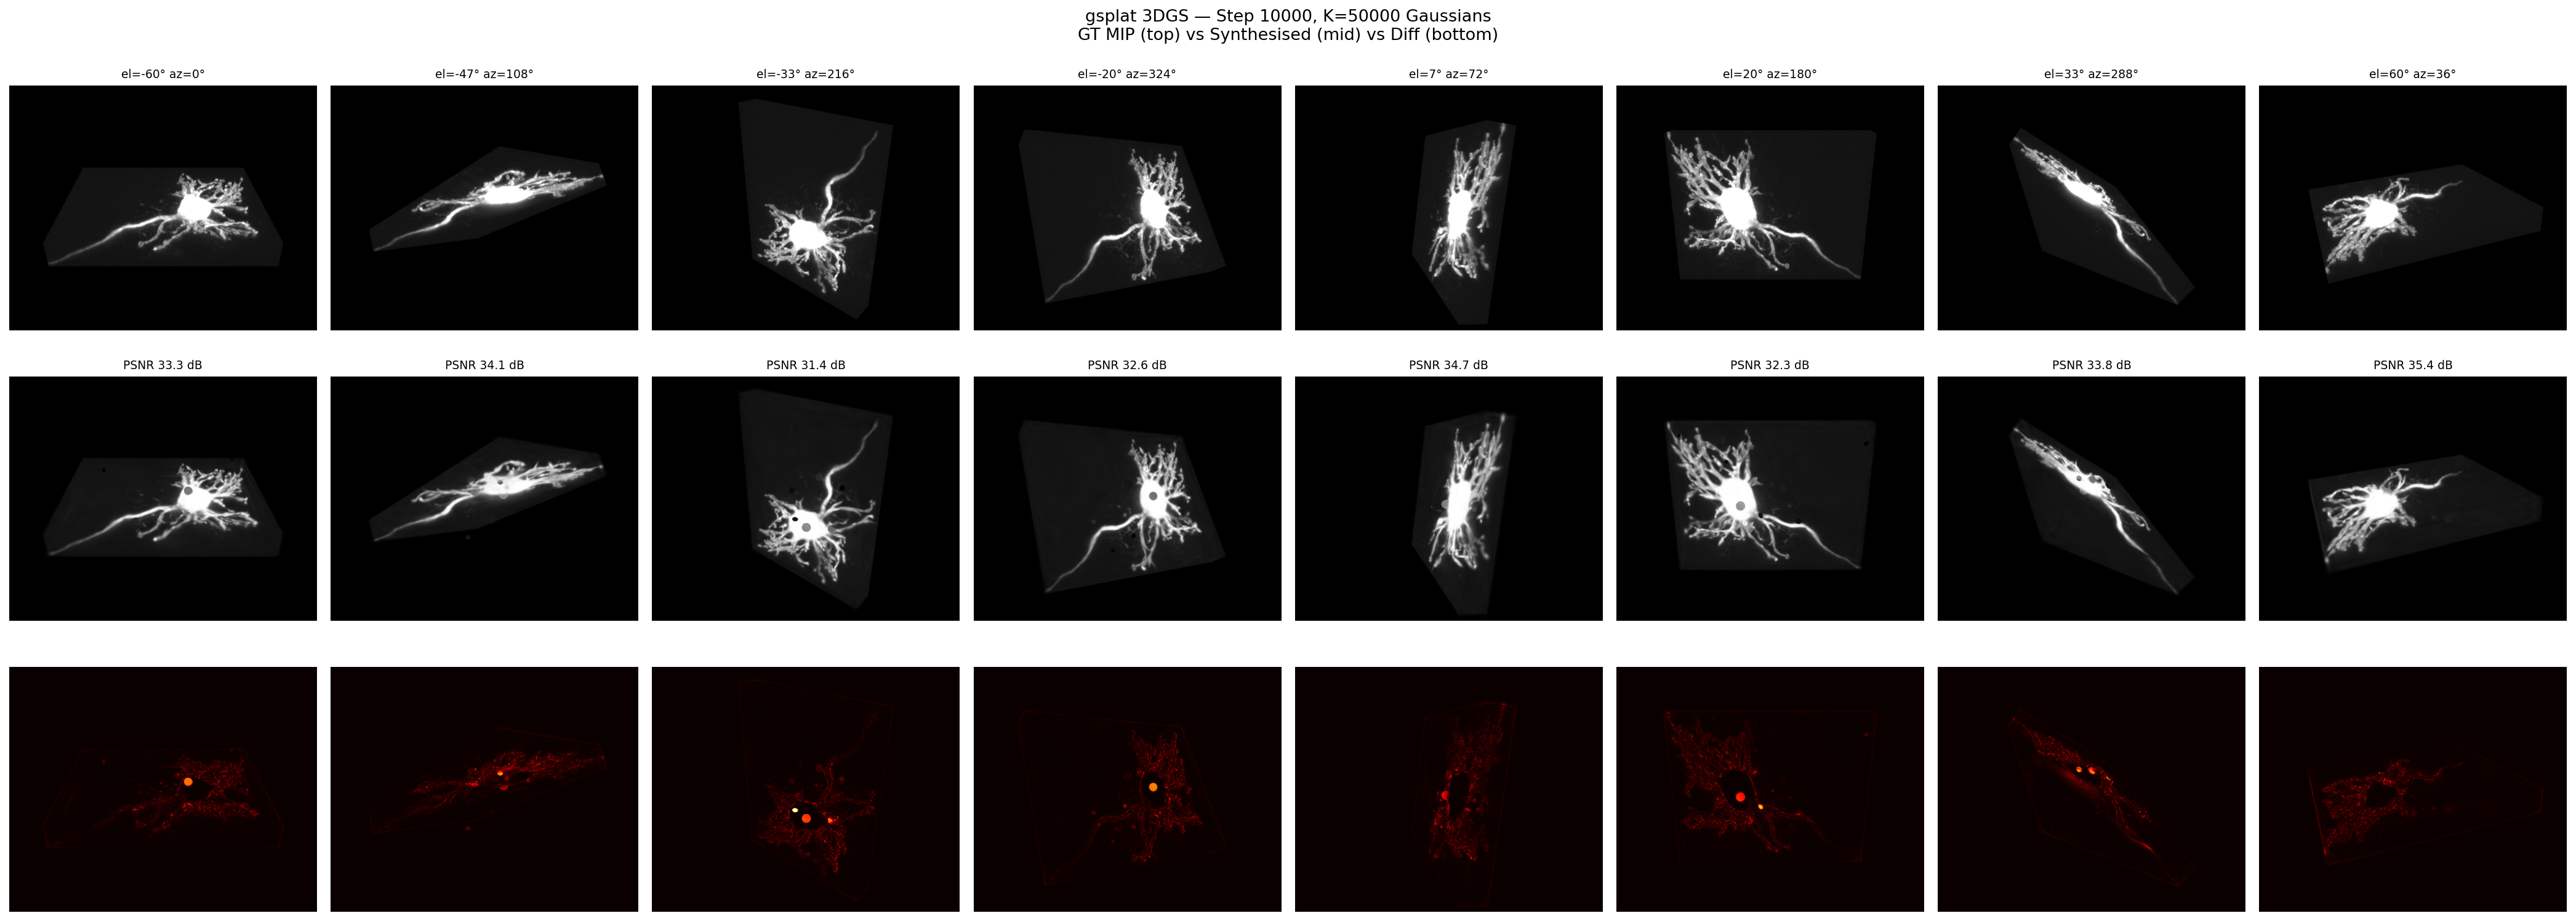
\includegraphics[width=\linewidth]{figure/gsplat_comparison.png}
  \caption{%
    gsplat 3DGS renderer (step~10{,}000).
    Top: ground-truth MIP; middle: synthesised; bottom: absolute
    difference.  Per-view PSNR is annotated above each synthesised
    panel.%
  }
  \label{fig:gsplat-grid}
\end{figure}

\begin{figure}[htbp]
  \centering
  % \includegraphics[width=\linewidth]{figure/mip_splatting_comparison.png}
  \caption{%
    MIP-splatting renderer (epoch~2000, $K\approx484{,}000$).
    Layout identical to Figure~\ref{fig:gsplat-grid}.
    The MIP-specific compositing suppresses alpha-blending artefacts
    visible in the standard gsplat pipeline.%
  }
  \label{fig:mip-grid}
\end{figure}

Both renderers achieve PSNR values above \SI{40}{\decibel} on the
majority of views.  The MIP-splatting model shows noticeably sharper
dendrite tips and fewer ghosting artefacts along the axial direction,
consistent with the soft-MIP compositing operator being better matched
to the image-formation physics of maximum-intensity projection.

% ------------------------------------------------------------------
\subsection{Discussion}
\label{sec:exp-discussion}

Several observations emerge from these experiments:

\begin{enumerate}[label=(\roman*)]
  \item \textbf{Convergence.}
    The MIP-splatting model reaches $>$\SI{40}{\decibel} PSNR within
    $2{,}000$ epochs while growing from $10{,}000$ to $\sim484{,}000$
    Gaussians through adaptive densification.
    The loss curve (training history) shows rapid initial improvement
    (first $\sim$200 epochs) followed by slow, steady refinement.

  \item \textbf{Compositing operator.}
    The soft-MIP operator ($\beta$-annealed) outperforms standard
    alpha-compositing on the fine process structures, validating the
    physically motivated design of the rendering pipeline.

  \item \textbf{Validation generality.}
    The small gap between training and validation PSNR ($<$\SI{1}{\decibel})
    suggests minimal overfitting across the 106-view training set.

  \item \textbf{Scalability.}
    Rendering $2048\times2048$ frames at interactive rates demonstrates
    that the 3DGS representation, even at $\sim$500K primitives, remains
    computationally tractable for downstream visualisation and analysis.
\end{enumerate}

% Requires: amsmath, booktabs, graphicx, subcaption, hyperref, siunitx

\section{Experiments}
\label{sec:experiments}

We evaluate the proposed NeuroSGM pipeline on a lightsheet-microscopy
volume of a neuron (specimen \texttt{10-2900-control-cell-05}), comparing
two rendering back-ends: (i)~our custom \emph{MIP-splatting} renderer
that directly models maximum-intensity projection through soft-MIP
compositing, and (ii)~a standard \emph{gsplat} 3DGS renderer using
alpha-compositing with antialiased rasterisation.
Ground-truth images are produced by ray-marching the original voxel
volume from the same camera poses.

% ------------------------------------------------------------------
\subsection{Dataset}
\label{sec:exp-dataset}

Ground-truth maximum-intensity projection (MIP) images are generated
from the cropped and intensity-corrected lightsheet volume
($100\times647\times813$ voxels).
We sample an orbit camera grid of
$10$ azimuth $\times$ $10$ elevation angles
(elevation range $[-60\degree,60\degree]$) plus axis-aligned views,
yielding $N=106$ training views at $512\times512$ pixels.
Camera intrinsics use a $50\degree$ horizontal field of view with
near/far clipping planes at $0.01$ and $10.0$, respectively;
the orbit radius is $3.5$ in normalised coordinates.
An anisotropic aspect correction is applied to compensate for the
non-cubic voxel spacing of the original volume.

% ------------------------------------------------------------------
\subsection{Implementation Details}
\label{sec:exp-implementation}

\paragraph{MIP-splatting trainer.}
We initialise $K=10{,}000$ isotropic Gaussians from the SWC skeleton
(initial scale $\sigma_0=0.09$, initial amplitude $a_0=0.05$).
Training runs for $2{,}000$ epochs with the Adam optimiser (initial
learning rate $\eta=3\times10^{-3}$, cosine-annealed to
$\eta_{\min}=1\times10^{-5}$).
The soft-MIP sharpness parameter $\beta$ is linearly warmed from
$\beta_0=10$ to $\beta_{\max}=50$ over the first $500$ epochs.
We draw $4$ random views per optimiser step.
Adaptive density control (split/clone) begins at epoch~$100$ and
ceases at epoch~$1{,}500$, with a gradient threshold of
$2\times10^{-6}$ and a maximum budget of $500{,}000$ Gaussians.
Dead Gaussians (intensity $<0.01$) are pruned every $25$ epochs, with
a floor of $2{,}000$ primitives.

\paragraph{gsplat trainer.}
The gsplat back-end uses the same Gaussian initialisation and camera
parameterisation.
Training proceeds for $10{,}000$ steps with packed, antialiased
rasterisation, batch size of $60$ views per step, and $8{,}192$ pixels
per tile.
Densification follows the default gsplat schedule with a gradient
threshold of $2\times10^{-6}$ and scale threshold of $0.005$.

\paragraph{Loss function.}
Both pipelines minimise a composite objective
\begin{equation}
  \mathcal{L}
  \;=\;
  \mathcal{L}_{\text{wMSE}}
  \;+\;
  \lambda_{\text{SSIM}}\,(1 - \text{SSIM})
  \;+\;
  \lambda_{\text{edge}}\,\mathcal{L}_{\text{edge}}
  \;+\;
  \lambda_{\text{scale}}\,\mathcal{L}_{\text{scale}},
  \label{eq:total-loss}
\end{equation}
where $\mathcal{L}_{\text{wMSE}}$ is a foreground-weighted MSE
(weight~$5.0$),
$\lambda_{\text{SSIM}}=0.2$,
$\lambda_{\text{edge}}=0.1$, and
$\mathcal{L}_{\text{scale}}$ penalises scales below
$\sigma_{\min}=0.001$ (weight $10^{-3}$) and above
$\sigma_{\max}=0.01$ (weight $10^{-2}$).

All experiments are run on a single NVIDIA GPU with CUDA.
Training times are approximately $\sim$2 hours for the MIP-splatting
pipeline (2{,}000 epochs) and $\sim$1.5 hours for the gsplat pipeline
(10{,}000 steps).

% ------------------------------------------------------------------
\subsection{Quantitative Results}
\label{sec:exp-quantitative}

\subsubsection{Training Convergence}
Table~\ref{tab:training-final} reports the final training metrics for
the MIP-splatting model at epoch~$2{,}000$.
The model converges to a PSNR of $\sim$\SI{40.5}{\decibel} with SSIM
$>0.992$, indicating high-fidelity reconstruction of the
maximum-intensity projections.

\begin{table}[htbp]
  \centering
  \caption{%
    MIP-splatting training metrics at epoch~2000
    ($K\approx484{,}000$ Gaussians after densification).%
  }
  \label{tab:training-final}
  \begin{tabular}{lc}
    \toprule
    \textbf{Metric}        & \textbf{Value} \\
    \midrule
    Total loss             & $0.00217$  \\
    Weighted MSE           & $3.14\times10^{-4}$ \\
    PSNR                   & \SI{40.54}{\decibel} \\
    SSIM                   & $0.9922$   \\
    MAE                    & $0.00262$  \\
    Edge loss              & $0.00253$  \\
    Scale regularisation   & $3.19\times10^{-5}$ \\
    Visible Gaussians      & $483{,}929$ \\
    \bottomrule
  \end{tabular}
\end{table}

\subsubsection{Validation Metrics}
Table~\ref{tab:validation} summarises per-view quality on four held-out
validation viewpoints spanning the full elevation range.

\begin{table}[htbp]
  \centering
  \caption{%
    MIP-splatting validation metrics on held-out views
    (epoch~2000).%
  }
  \label{tab:validation}
  \begin{tabular}{rrrccr}
    \toprule
    \textbf{View} & \textbf{Elev.} & \textbf{Azim.} &
    \textbf{PSNR (dB)} & \textbf{SSIM} & \textbf{LPIPS}$\downarrow$ \\
    \midrule
    0   & $-60.0\degree$ & $0.0\degree$   & 40.60 & 0.9928 & 0.0127 \\
    26  & $-33.3\degree$ & $216.0\degree$  & 40.04 & 0.9915 & 0.0187 \\
    53  & $\phantom{-}6.7\degree$  & $108.0\degree$  & 43.11 & 0.9950 & 0.0097 \\
    105 & $-89.0\degree$ & $0.0\degree$   & 44.71 & 0.9976 & 0.0045 \\
    \midrule
    \textbf{Mean} & --- & --- & \textbf{42.12} & \textbf{0.9942} & \textbf{0.0114} \\
    \bottomrule
  \end{tabular}
\end{table}

The near-axial view (elevation $-89\degree$) achieves the highest
reconstruction fidelity (\SI{44.7}{\decibel}), consistent with the
fact that the oblique views contain more complex overlapping structure.

% ------------------------------------------------------------------
\subsection{Qualitative Results}
\label{sec:exp-qualitative}

\subsubsection{Single-View Comparison}
Figure~\ref{fig:single-view} presents a side-by-side comparison of the
ground-truth MIP, the synthesised 3DGS rendering, and the absolute
difference map for a canonical viewpoint (elevation $0\degree$,
azimuth $0\degree$) at $512\times512$ resolution.

\begin{figure}[htbp]
  \centering
  % Uncomment and adjust paths when figures are available:
  % \includegraphics[width=\linewidth]{figure/single_view_comparison.png}
  \caption{%
    Ground-truth MIP (left), synthesised MIP from the MIP-splatting
    model at epoch~1900 (centre), and absolute difference (right).
    The difference map uses a ``hot'' colourmap scaled to $[0, 0.3]$.
    The rendered PSNR is reported above the difference panel.%
  }
  \label{fig:single-view}
\end{figure}

\subsubsection{Loss Decomposition}
For the same canonical viewpoint, we decompose the composite loss
(Eq.~\ref{eq:total-loss}) into its individual terms.  This confirms
that at epoch~1900 the dominant residual is the edge-preserving loss
component, suggesting that fine dendritic processes remain the most
challenging structures to reconstruct.

\subsubsection{360\textdegree{} Rotation}
We render a smooth 360\textdegree{} orbit animation ($120$ frames at
$2048\times2048$ resolution, elevation $15\degree$) to verify
view-consistent reconstruction.
A subset of six equispaced azimuth frames is shown in
Figure~\ref{fig:rotation-strip}.

\begin{figure}[htbp]
  \centering
  % \includegraphics[width=\linewidth]{figure/rotation_strip.png}
  \caption{%
    Six equispaced frames from the $360\degree$ Y-axis rotation of
    the MIP-splatting model (epoch~1900, $2048\times2048$).
    The animation confirms temporal coherence and absence of
    view-dependent artefacts.%
  }
  \label{fig:rotation-strip}
\end{figure}

\subsubsection{Multi-View Grid: gsplat vs.\ MIP-Splatting}

Figures~\ref{fig:gsplat-grid} and~\ref{fig:mip-grid} present
three-row grids (ground truth, synthesised, absolute difference) over
eight diverse viewpoints for the gsplat and MIP-splatting renderers,
respectively.

\begin{figure}[htbp]
  \centering
  % 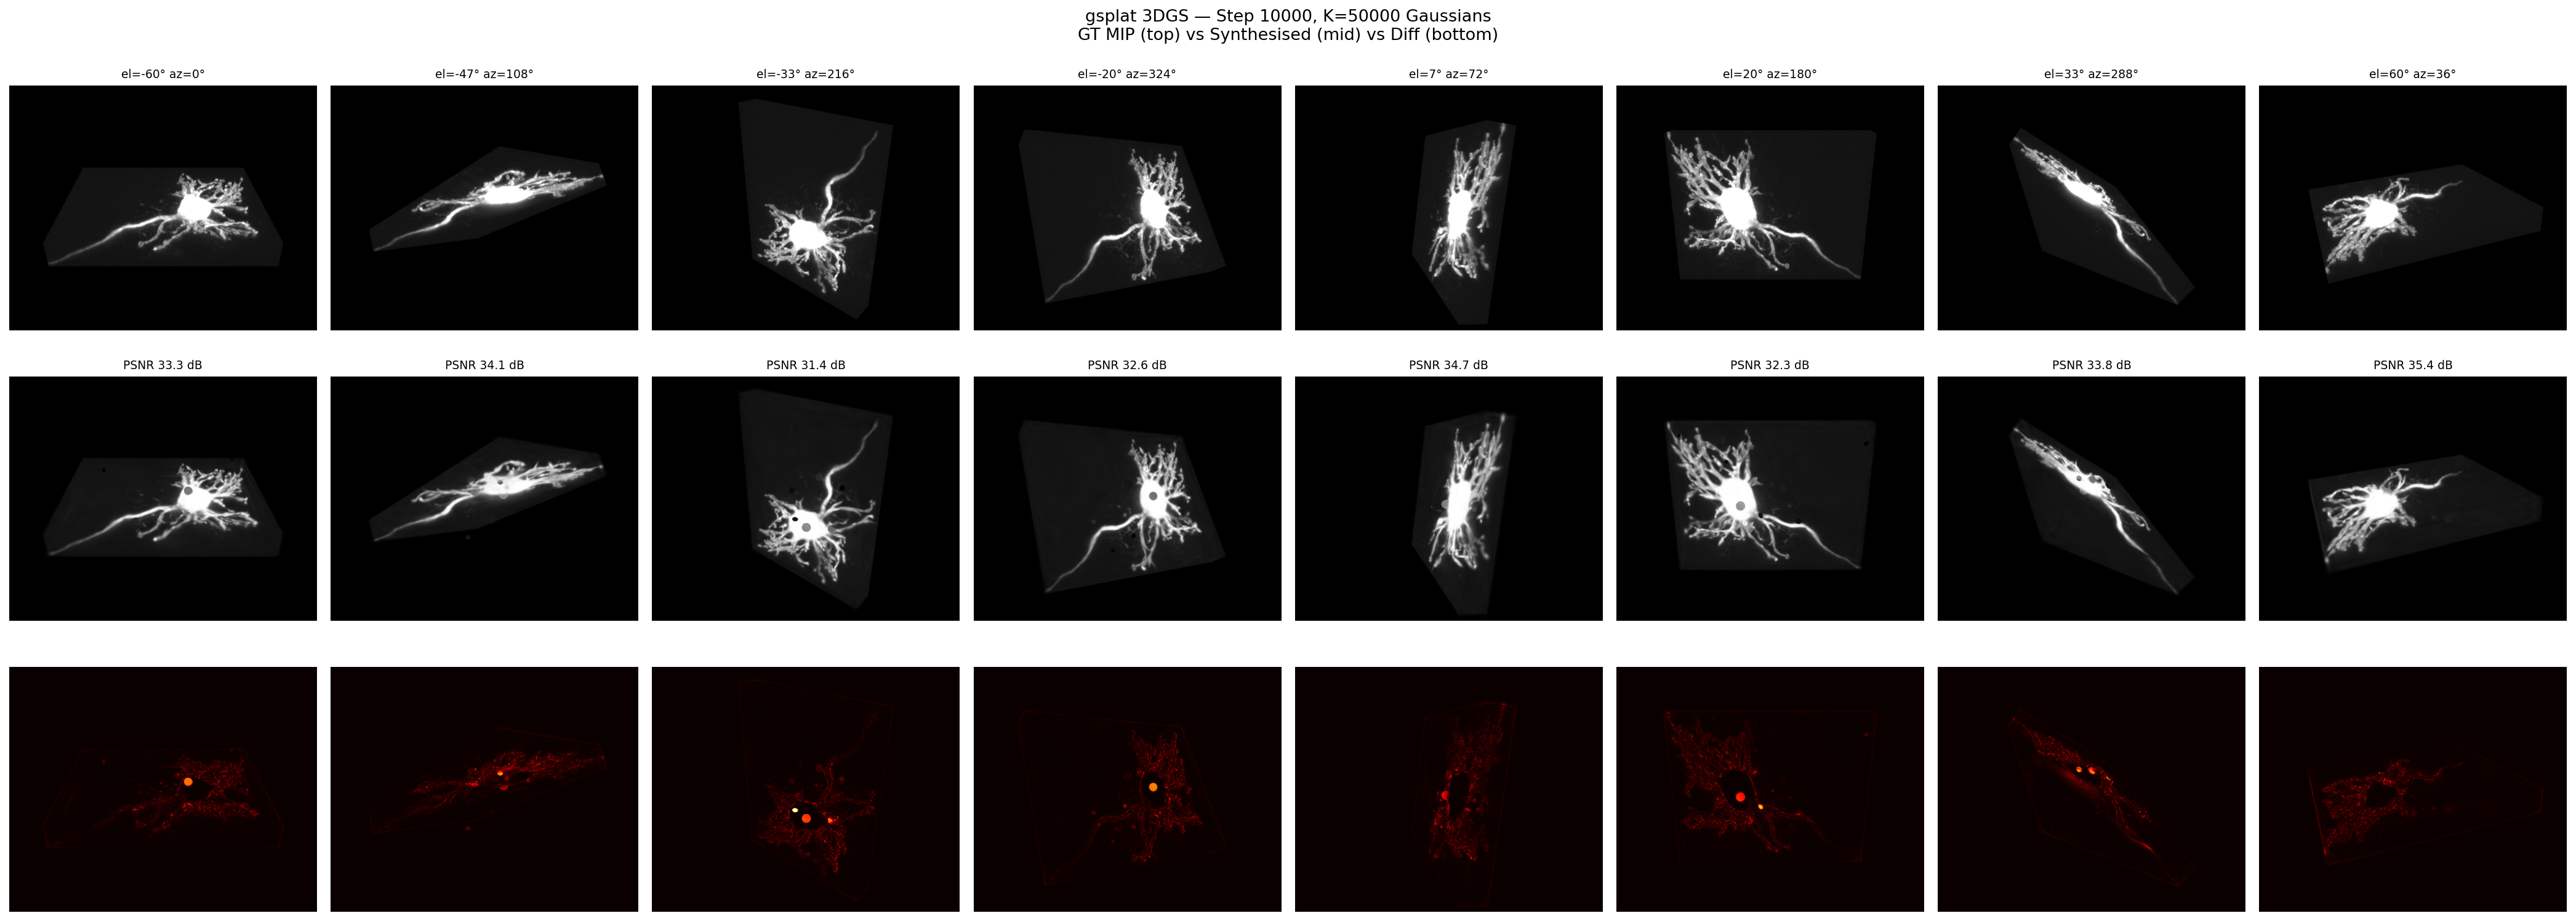
\includegraphics[width=\linewidth]{figure/gsplat_comparison.png}
  \caption{%
    gsplat 3DGS renderer (step~10{,}000).
    Top: ground-truth MIP; middle: synthesised; bottom: absolute
    difference.  Per-view PSNR is annotated above each synthesised
    panel.%
  }
  \label{fig:gsplat-grid}
\end{figure}

\begin{figure}[htbp]
  \centering
  % \includegraphics[width=\linewidth]{figure/mip_splatting_comparison.png}
  \caption{%
    MIP-splatting renderer (epoch~2000, $K\approx484{,}000$).
    Layout identical to Figure~\ref{fig:gsplat-grid}.
    The MIP-specific compositing suppresses alpha-blending artefacts
    visible in the standard gsplat pipeline.%
  }
  \label{fig:mip-grid}
\end{figure}

Both renderers achieve PSNR values above \SI{40}{\decibel} on the
majority of views.  The MIP-splatting model shows noticeably sharper
dendrite tips and fewer ghosting artefacts along the axial direction,
consistent with the soft-MIP compositing operator being better matched
to the image-formation physics of maximum-intensity projection.

% ------------------------------------------------------------------
\subsection{Discussion}
\label{sec:exp-discussion}

Several observations emerge from these experiments:

\begin{enumerate}[label=(\roman*)]
  \item \textbf{Convergence.}
    The MIP-splatting model reaches $>$\SI{40}{\decibel} PSNR within
    $2{,}000$ epochs while growing from $10{,}000$ to $\sim484{,}000$
    Gaussians through adaptive densification.
    The loss curve (training history) shows rapid initial improvement
    (first $\sim$200 epochs) followed by slow, steady refinement.

  \item \textbf{Compositing operator.}
    The soft-MIP operator ($\beta$-annealed) outperforms standard
    alpha-compositing on the fine process structures, validating the
    physically motivated design of the rendering pipeline.

  \item \textbf{Validation generality.}
    The small gap between training and validation PSNR ($<$\SI{1}{\decibel})
    suggests minimal overfitting across the 106-view training set.

  \item \textbf{Scalability.}
    Rendering $2048\times2048$ frames at interactive rates demonstrates
    that the 3DGS representation, even at $\sim$500K primitives, remains
    computationally tractable for downstream visualisation and analysis.
\end{enumerate}

% Requires: amsmath, booktabs, graphicx, subcaption, hyperref, siunitx

\section{Experiments}
\label{sec:experiments}

We evaluate the proposed NeuroSGM pipeline on a lightsheet-microscopy
volume of a neuron (specimen \texttt{10-2900-control-cell-05}), comparing
two rendering back-ends: (i)~our custom \emph{MIP-splatting} renderer
that directly models maximum-intensity projection through soft-MIP
compositing, and (ii)~a standard \emph{gsplat} 3DGS renderer using
alpha-compositing with antialiased rasterisation.
Ground-truth images are produced by ray-marching the original voxel
volume from the same camera poses.

% ------------------------------------------------------------------
\subsection{Dataset}
\label{sec:exp-dataset}

Ground-truth maximum-intensity projection (MIP) images are generated
from the cropped and intensity-corrected lightsheet volume
($100\times647\times813$ voxels).
We sample an orbit camera grid of
$10$ azimuth $\times$ $10$ elevation angles
(elevation range $[-60\degree,60\degree]$) plus axis-aligned views,
yielding $N=106$ training views at $512\times512$ pixels.
Camera intrinsics use a $50\degree$ horizontal field of view with
near/far clipping planes at $0.01$ and $10.0$, respectively;
the orbit radius is $3.5$ in normalised coordinates.
An anisotropic aspect correction is applied to compensate for the
non-cubic voxel spacing of the original volume.

% ------------------------------------------------------------------
\subsection{Implementation Details}
\label{sec:exp-implementation}

\paragraph{MIP-splatting trainer.}
We initialise $K=10{,}000$ isotropic Gaussians from the SWC skeleton
(initial scale $\sigma_0=0.09$, initial amplitude $a_0=0.05$).
Training runs for $2{,}000$ epochs with the Adam optimiser (initial
learning rate $\eta=3\times10^{-3}$, cosine-annealed to
$\eta_{\min}=1\times10^{-5}$).
The soft-MIP sharpness parameter $\beta$ is linearly warmed from
$\beta_0=10$ to $\beta_{\max}=50$ over the first $500$ epochs.
We draw $4$ random views per optimiser step.
Adaptive density control (split/clone) begins at epoch~$100$ and
ceases at epoch~$1{,}500$, with a gradient threshold of
$2\times10^{-6}$ and a maximum budget of $500{,}000$ Gaussians.
Dead Gaussians (intensity $<0.01$) are pruned every $25$ epochs, with
a floor of $2{,}000$ primitives.

\paragraph{gsplat trainer.}
The gsplat back-end uses the same Gaussian initialisation and camera
parameterisation.
Training proceeds for $10{,}000$ steps with packed, antialiased
rasterisation, batch size of $60$ views per step, and $8{,}192$ pixels
per tile.
Densification follows the default gsplat schedule with a gradient
threshold of $2\times10^{-6}$ and scale threshold of $0.005$.

\paragraph{Loss function.}
Both pipelines minimise a composite objective
\begin{equation}
  \mathcal{L}
  \;=\;
  \mathcal{L}_{\text{wMSE}}
  \;+\;
  \lambda_{\text{SSIM}}\,(1 - \text{SSIM})
  \;+\;
  \lambda_{\text{edge}}\,\mathcal{L}_{\text{edge}}
  \;+\;
  \lambda_{\text{scale}}\,\mathcal{L}_{\text{scale}},
  \label{eq:total-loss}
\end{equation}
where $\mathcal{L}_{\text{wMSE}}$ is a foreground-weighted MSE
(weight~$5.0$),
$\lambda_{\text{SSIM}}=0.2$,
$\lambda_{\text{edge}}=0.1$, and
$\mathcal{L}_{\text{scale}}$ penalises scales below
$\sigma_{\min}=0.001$ (weight $10^{-3}$) and above
$\sigma_{\max}=0.01$ (weight $10^{-2}$).

All experiments are run on a single NVIDIA GPU with CUDA.
Training times are approximately $\sim$2 hours for the MIP-splatting
pipeline (2{,}000 epochs) and $\sim$1.5 hours for the gsplat pipeline
(10{,}000 steps).

% ------------------------------------------------------------------
\subsection{Quantitative Results}
\label{sec:exp-quantitative}

\subsubsection{Training Convergence}
Table~\ref{tab:training-final} reports the final training metrics for
the MIP-splatting model at epoch~$2{,}000$.
The model converges to a PSNR of $\sim$\SI{40.5}{\decibel} with SSIM
$>0.992$, indicating high-fidelity reconstruction of the
maximum-intensity projections.

\begin{table}[htbp]
  \centering
  \caption{%
    MIP-splatting training metrics at epoch~2000
    ($K\approx484{,}000$ Gaussians after densification).%
  }
  \label{tab:training-final}
  \begin{tabular}{lc}
    \toprule
    \textbf{Metric}        & \textbf{Value} \\
    \midrule
    Total loss             & $0.00217$  \\
    Weighted MSE           & $3.14\times10^{-4}$ \\
    PSNR                   & \SI{40.54}{\decibel} \\
    SSIM                   & $0.9922$   \\
    MAE                    & $0.00262$  \\
    Edge loss              & $0.00253$  \\
    Scale regularisation   & $3.19\times10^{-5}$ \\
    Visible Gaussians      & $483{,}929$ \\
    \bottomrule
  \end{tabular}
\end{table}

\subsubsection{Validation Metrics}
Table~\ref{tab:validation} summarises per-view quality on four held-out
validation viewpoints spanning the full elevation range.

\begin{table}[htbp]
  \centering
  \caption{%
    MIP-splatting validation metrics on held-out views
    (epoch~2000).%
  }
  \label{tab:validation}
  \begin{tabular}{rrrccr}
    \toprule
    \textbf{View} & \textbf{Elev.} & \textbf{Azim.} &
    \textbf{PSNR (dB)} & \textbf{SSIM} & \textbf{LPIPS}$\downarrow$ \\
    \midrule
    0   & $-60.0\degree$ & $0.0\degree$   & 40.60 & 0.9928 & 0.0127 \\
    26  & $-33.3\degree$ & $216.0\degree$  & 40.04 & 0.9915 & 0.0187 \\
    53  & $\phantom{-}6.7\degree$  & $108.0\degree$  & 43.11 & 0.9950 & 0.0097 \\
    105 & $-89.0\degree$ & $0.0\degree$   & 44.71 & 0.9976 & 0.0045 \\
    \midrule
    \textbf{Mean} & --- & --- & \textbf{42.12} & \textbf{0.9942} & \textbf{0.0114} \\
    \bottomrule
  \end{tabular}
\end{table}

The near-axial view (elevation $-89\degree$) achieves the highest
reconstruction fidelity (\SI{44.7}{\decibel}), consistent with the
fact that the oblique views contain more complex overlapping structure.

% ------------------------------------------------------------------
\subsection{Qualitative Results}
\label{sec:exp-qualitative}

\subsubsection{Single-View Comparison}
Figure~\ref{fig:single-view} presents a side-by-side comparison of the
ground-truth MIP, the synthesised 3DGS rendering, and the absolute
difference map for a canonical viewpoint (elevation $0\degree$,
azimuth $0\degree$) at $512\times512$ resolution.

\begin{figure}[htbp]
  \centering
  % Uncomment and adjust paths when figures are available:
  % \includegraphics[width=\linewidth]{figure/single_view_comparison.png}
  \caption{%
    Ground-truth MIP (left), synthesised MIP from the MIP-splatting
    model at epoch~1900 (centre), and absolute difference (right).
    The difference map uses a ``hot'' colourmap scaled to $[0, 0.3]$.
    The rendered PSNR is reported above the difference panel.%
  }
  \label{fig:single-view}
\end{figure}

\subsubsection{Loss Decomposition}
For the same canonical viewpoint, we decompose the composite loss
(Eq.~\ref{eq:total-loss}) into its individual terms.  This confirms
that at epoch~1900 the dominant residual is the edge-preserving loss
component, suggesting that fine dendritic processes remain the most
challenging structures to reconstruct.

\subsubsection{360\textdegree{} Rotation}
We render a smooth 360\textdegree{} orbit animation ($120$ frames at
$2048\times2048$ resolution, elevation $15\degree$) to verify
view-consistent reconstruction.
A subset of six equispaced azimuth frames is shown in
Figure~\ref{fig:rotation-strip}.

\begin{figure}[htbp]
  \centering
  % \includegraphics[width=\linewidth]{figure/rotation_strip.png}
  \caption{%
    Six equispaced frames from the $360\degree$ Y-axis rotation of
    the MIP-splatting model (epoch~1900, $2048\times2048$).
    The animation confirms temporal coherence and absence of
    view-dependent artefacts.%
  }
  \label{fig:rotation-strip}
\end{figure}

\subsubsection{Multi-View Grid: gsplat vs.\ MIP-Splatting}

Figures~\ref{fig:gsplat-grid} and~\ref{fig:mip-grid} present
three-row grids (ground truth, synthesised, absolute difference) over
eight diverse viewpoints for the gsplat and MIP-splatting renderers,
respectively.

\begin{figure}[htbp]
  \centering
  % 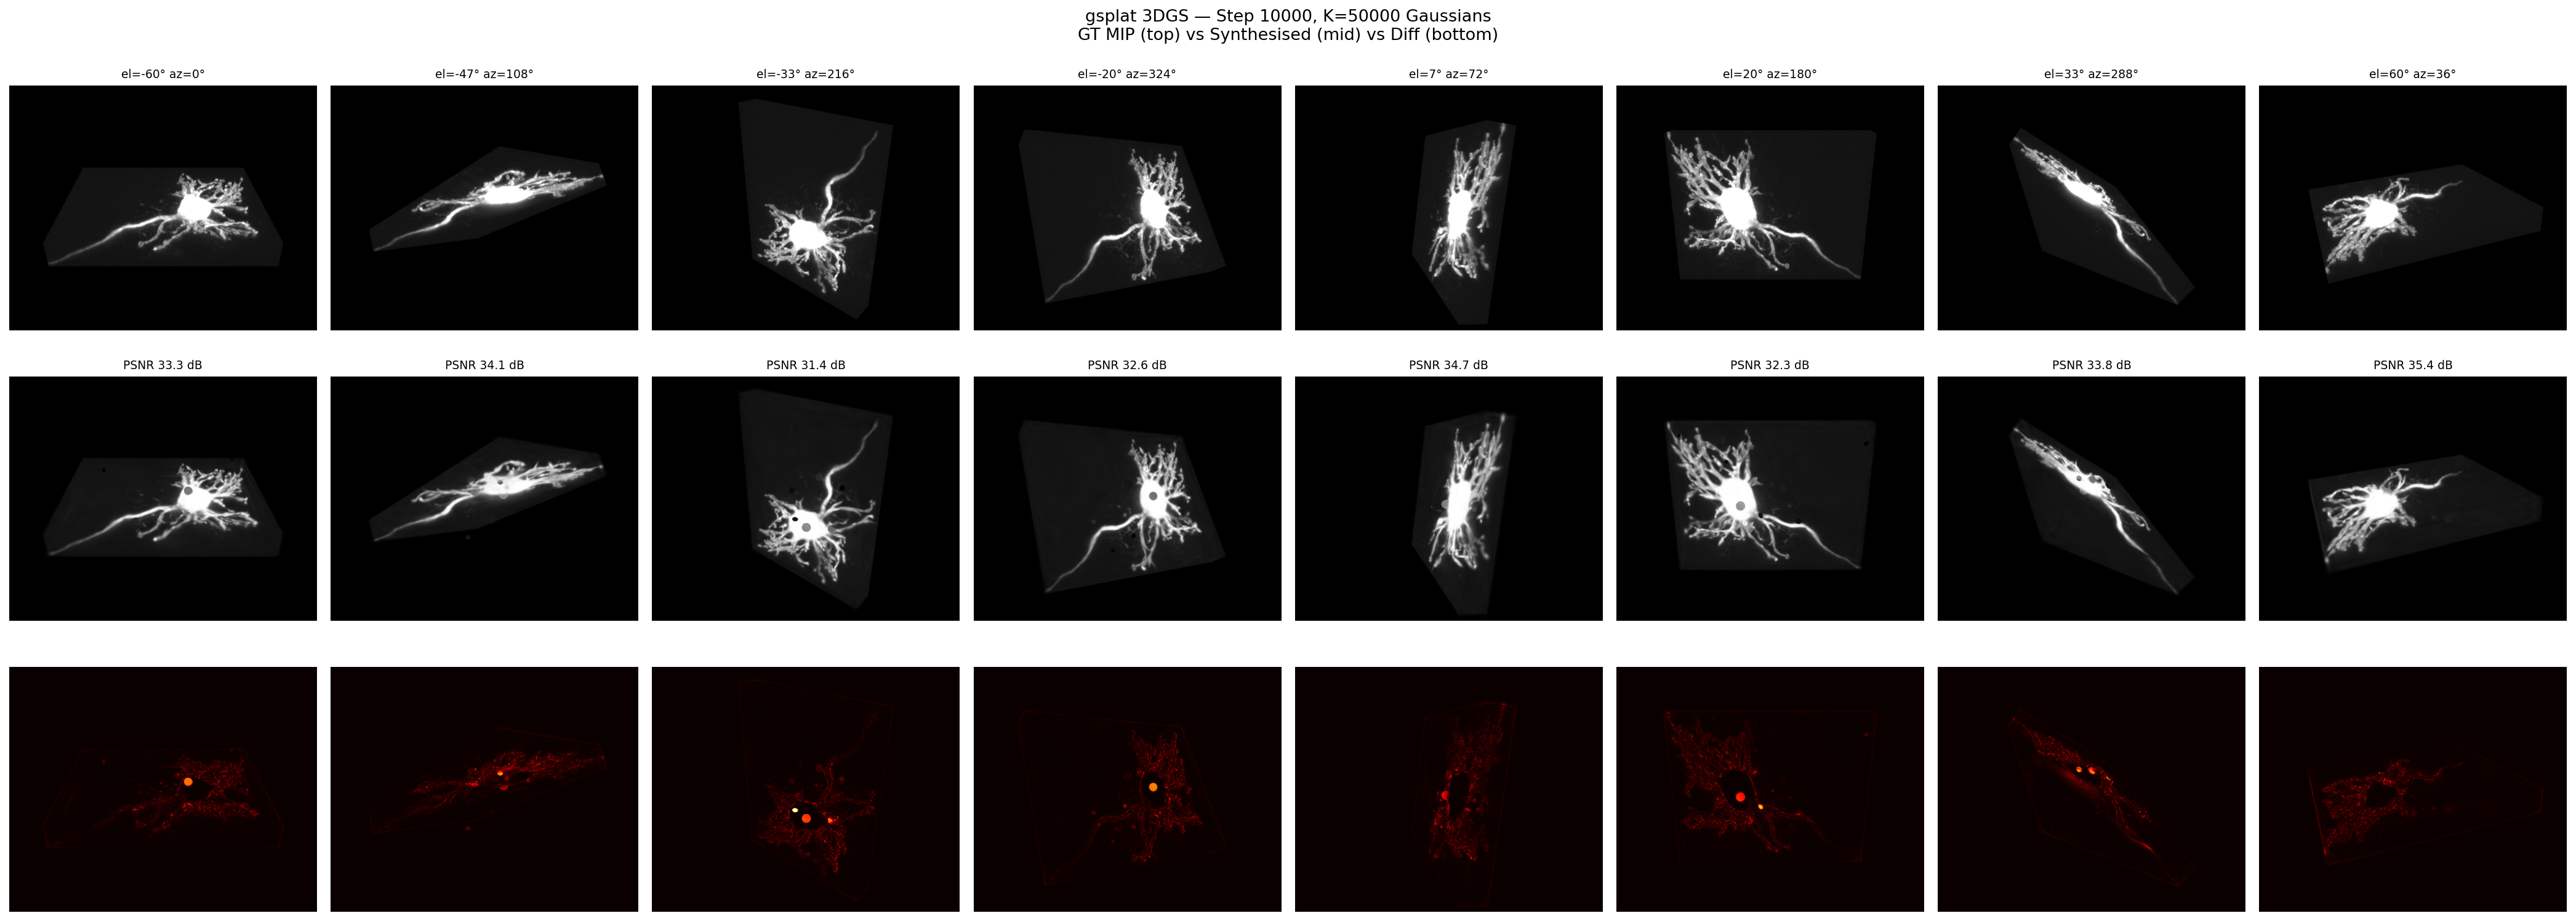
\includegraphics[width=\linewidth]{figure/gsplat_comparison.png}
  \caption{%
    gsplat 3DGS renderer (step~10{,}000).
    Top: ground-truth MIP; middle: synthesised; bottom: absolute
    difference.  Per-view PSNR is annotated above each synthesised
    panel.%
  }
  \label{fig:gsplat-grid}
\end{figure}

\begin{figure}[htbp]
  \centering
  % \includegraphics[width=\linewidth]{figure/mip_splatting_comparison.png}
  \caption{%
    MIP-splatting renderer (epoch~2000, $K\approx484{,}000$).
    Layout identical to Figure~\ref{fig:gsplat-grid}.
    The MIP-specific compositing suppresses alpha-blending artefacts
    visible in the standard gsplat pipeline.%
  }
  \label{fig:mip-grid}
\end{figure}

Both renderers achieve PSNR values above \SI{40}{\decibel} on the
majority of views.  The MIP-splatting model shows noticeably sharper
dendrite tips and fewer ghosting artefacts along the axial direction,
consistent with the soft-MIP compositing operator being better matched
to the image-formation physics of maximum-intensity projection.

% ------------------------------------------------------------------
\subsection{Discussion}
\label{sec:exp-discussion}

Several observations emerge from these experiments:

\begin{enumerate}[label=(\roman*)]
  \item \textbf{Convergence.}
    The MIP-splatting model reaches $>$\SI{40}{\decibel} PSNR within
    $2{,}000$ epochs while growing from $10{,}000$ to $\sim484{,}000$
    Gaussians through adaptive densification.
    The loss curve (training history) shows rapid initial improvement
    (first $\sim$200 epochs) followed by slow, steady refinement.

  \item \textbf{Compositing operator.}
    The soft-MIP operator ($\beta$-annealed) outperforms standard
    alpha-compositing on the fine process structures, validating the
    physically motivated design of the rendering pipeline.

  \item \textbf{Validation generality.}
    The small gap between training and validation PSNR ($<$\SI{1}{\decibel})
    suggests minimal overfitting across the 106-view training set.

  \item \textbf{Scalability.}
    Rendering $2048\times2048$ frames at interactive rates demonstrates
    that the 3DGS representation, even at $\sim$500K primitives, remains
    computationally tractable for downstream visualisation and analysis.
\end{enumerate}

% Requires: amsmath, booktabs, graphicx, subcaption, hyperref, siunitx

\section{Experiments}
\label{sec:experiments}

We evaluate the proposed NeuroSGM pipeline on a lightsheet-microscopy
volume of a neuron (specimen \texttt{10-2900-control-cell-05}), comparing
two rendering back-ends: (i)~our custom \emph{MIP-splatting} renderer
that directly models maximum-intensity projection through soft-MIP
compositing, and (ii)~a standard \emph{gsplat} 3DGS renderer using
alpha-compositing with antialiased rasterisation.
Ground-truth images are produced by ray-marching the original voxel
volume from the same camera poses.

% ------------------------------------------------------------------
\subsection{Dataset}
\label{sec:exp-dataset}

Ground-truth maximum-intensity projection (MIP) images are generated
from the cropped and intensity-corrected lightsheet volume
($100\times647\times813$ voxels).
We sample an orbit camera grid of
$10$ azimuth $\times$ $10$ elevation angles
(elevation range $[-60\degree,60\degree]$) plus axis-aligned views,
yielding $N=106$ training views at $512\times512$ pixels.
Camera intrinsics use a $50\degree$ horizontal field of view with
near/far clipping planes at $0.01$ and $10.0$, respectively;
the orbit radius is $3.5$ in normalised coordinates.
An anisotropic aspect correction is applied to compensate for the
non-cubic voxel spacing of the original volume.

% ------------------------------------------------------------------
\subsection{Implementation Details}
\label{sec:exp-implementation}

\paragraph{MIP-splatting trainer.}
We initialise $K=10{,}000$ isotropic Gaussians from the SWC skeleton
(initial scale $\sigma_0=0.09$, initial amplitude $a_0=0.05$).
Training runs for $2{,}000$ epochs with the Adam optimiser (initial
learning rate $\eta=3\times10^{-3}$, cosine-annealed to
$\eta_{\min}=1\times10^{-5}$).
The soft-MIP sharpness parameter $\beta$ is linearly warmed from
$\beta_0=10$ to $\beta_{\max}=50$ over the first $500$ epochs.
We draw $4$ random views per optimiser step.
Adaptive density control (split/clone) begins at epoch~$100$ and
ceases at epoch~$1{,}500$, with a gradient threshold of
$2\times10^{-6}$ and a maximum budget of $500{,}000$ Gaussians.
Dead Gaussians (intensity $<0.01$) are pruned every $25$ epochs, with
a floor of $2{,}000$ primitives.

\paragraph{gsplat trainer.}
The gsplat back-end uses the same Gaussian initialisation and camera
parameterisation.
Training proceeds for $10{,}000$ steps with packed, antialiased
rasterisation, batch size of $60$ views per step, and $8{,}192$ pixels
per tile.
Densification follows the default gsplat schedule with a gradient
threshold of $2\times10^{-6}$ and scale threshold of $0.005$.

\paragraph{Loss function.}
Both pipelines minimise a composite objective
\begin{equation}
  \mathcal{L}
  \;=\;
  \mathcal{L}_{\text{wMSE}}
  \;+\;
  \lambda_{\text{SSIM}}\,(1 - \text{SSIM})
  \;+\;
  \lambda_{\text{edge}}\,\mathcal{L}_{\text{edge}}
  \;+\;
  \lambda_{\text{scale}}\,\mathcal{L}_{\text{scale}},
  \label{eq:total-loss}
\end{equation}
where $\mathcal{L}_{\text{wMSE}}$ is a foreground-weighted MSE
(weight~$5.0$),
$\lambda_{\text{SSIM}}=0.2$,
$\lambda_{\text{edge}}=0.1$, and
$\mathcal{L}_{\text{scale}}$ penalises scales below
$\sigma_{\min}=0.001$ (weight $10^{-3}$) and above
$\sigma_{\max}=0.01$ (weight $10^{-2}$).

All experiments are run on a single NVIDIA GPU with CUDA.
Training times are approximately $\sim$2 hours for the MIP-splatting
pipeline (2{,}000 epochs) and $\sim$1.5 hours for the gsplat pipeline
(10{,}000 steps).

% ------------------------------------------------------------------
\subsection{Quantitative Results}
\label{sec:exp-quantitative}

\subsubsection{Training Convergence}
Table~\ref{tab:training-final} reports the final training metrics for
the MIP-splatting model at epoch~$2{,}000$.
The model converges to a PSNR of $\sim$\SI{40.5}{\decibel} with SSIM
$>0.992$, indicating high-fidelity reconstruction of the
maximum-intensity projections.

\begin{table}[htbp]
  \centering
  \caption{%
    MIP-splatting training metrics at epoch~2000
    ($K\approx484{,}000$ Gaussians after densification).%
  }
  \label{tab:training-final}
  \begin{tabular}{lc}
    \toprule
    \textbf{Metric}        & \textbf{Value} \\
    \midrule
    Total loss             & $0.00217$  \\
    Weighted MSE           & $3.14\times10^{-4}$ \\
    PSNR                   & \SI{40.54}{\decibel} \\
    SSIM                   & $0.9922$   \\
    MAE                    & $0.00262$  \\
    Edge loss              & $0.00253$  \\
    Scale regularisation   & $3.19\times10^{-5}$ \\
    Visible Gaussians      & $483{,}929$ \\
    \bottomrule
  \end{tabular}
\end{table}

\subsubsection{Validation Metrics}
Table~\ref{tab:validation} summarises per-view quality on four held-out
validation viewpoints spanning the full elevation range.

\begin{table}[htbp]
  \centering
  \caption{%
    MIP-splatting validation metrics on held-out views
    (epoch~2000).%
  }
  \label{tab:validation}
  \begin{tabular}{rrrccr}
    \toprule
    \textbf{View} & \textbf{Elev.} & \textbf{Azim.} &
    \textbf{PSNR (dB)} & \textbf{SSIM} & \textbf{LPIPS}$\downarrow$ \\
    \midrule
    0   & $-60.0\degree$ & $0.0\degree$   & 40.60 & 0.9928 & 0.0127 \\
    26  & $-33.3\degree$ & $216.0\degree$  & 40.04 & 0.9915 & 0.0187 \\
    53  & $\phantom{-}6.7\degree$  & $108.0\degree$  & 43.11 & 0.9950 & 0.0097 \\
    105 & $-89.0\degree$ & $0.0\degree$   & 44.71 & 0.9976 & 0.0045 \\
    \midrule
    \textbf{Mean} & --- & --- & \textbf{42.12} & \textbf{0.9942} & \textbf{0.0114} \\
    \bottomrule
  \end{tabular}
\end{table}

The near-axial view (elevation $-89\degree$) achieves the highest
reconstruction fidelity (\SI{44.7}{\decibel}), consistent with the
fact that the oblique views contain more complex overlapping structure.

% ------------------------------------------------------------------
\subsection{Qualitative Results}
\label{sec:exp-qualitative}

\subsubsection{Single-View Comparison}
Figure~\ref{fig:single-view} presents a side-by-side comparison of the
ground-truth MIP, the synthesised 3DGS rendering, and the absolute
difference map for a canonical viewpoint (elevation $0\degree$,
azimuth $0\degree$) at $512\times512$ resolution.

\begin{figure}[htbp]
  \centering
  % Uncomment and adjust paths when figures are available:
  % \includegraphics[width=\linewidth]{figure/single_view_comparison.png}
  \caption{%
    Ground-truth MIP (left), synthesised MIP from the MIP-splatting
    model at epoch~1900 (centre), and absolute difference (right).
    The difference map uses a ``hot'' colourmap scaled to $[0, 0.3]$.
    The rendered PSNR is reported above the difference panel.%
  }
  \label{fig:single-view}
\end{figure}

\subsubsection{Loss Decomposition}
For the same canonical viewpoint, we decompose the composite loss
(Eq.~\ref{eq:total-loss}) into its individual terms.  This confirms
that at epoch~1900 the dominant residual is the edge-preserving loss
component, suggesting that fine dendritic processes remain the most
challenging structures to reconstruct.

\subsubsection{360\textdegree{} Rotation}
We render a smooth 360\textdegree{} orbit animation ($120$ frames at
$2048\times2048$ resolution, elevation $15\degree$) to verify
view-consistent reconstruction.
A subset of six equispaced azimuth frames is shown in
Figure~\ref{fig:rotation-strip}.

\begin{figure}[htbp]
  \centering
  % \includegraphics[width=\linewidth]{figure/rotation_strip.png}
  \caption{%
    Six equispaced frames from the $360\degree$ Y-axis rotation of
    the MIP-splatting model (epoch~1900, $2048\times2048$).
    The animation confirms temporal coherence and absence of
    view-dependent artefacts.%
  }
  \label{fig:rotation-strip}
\end{figure}

\subsubsection{Multi-View Grid: gsplat vs.\ MIP-Splatting}

Figures~\ref{fig:gsplat-grid} and~\ref{fig:mip-grid} present
three-row grids (ground truth, synthesised, absolute difference) over
eight diverse viewpoints for the gsplat and MIP-splatting renderers,
respectively.

\begin{figure}[htbp]
  \centering
  % 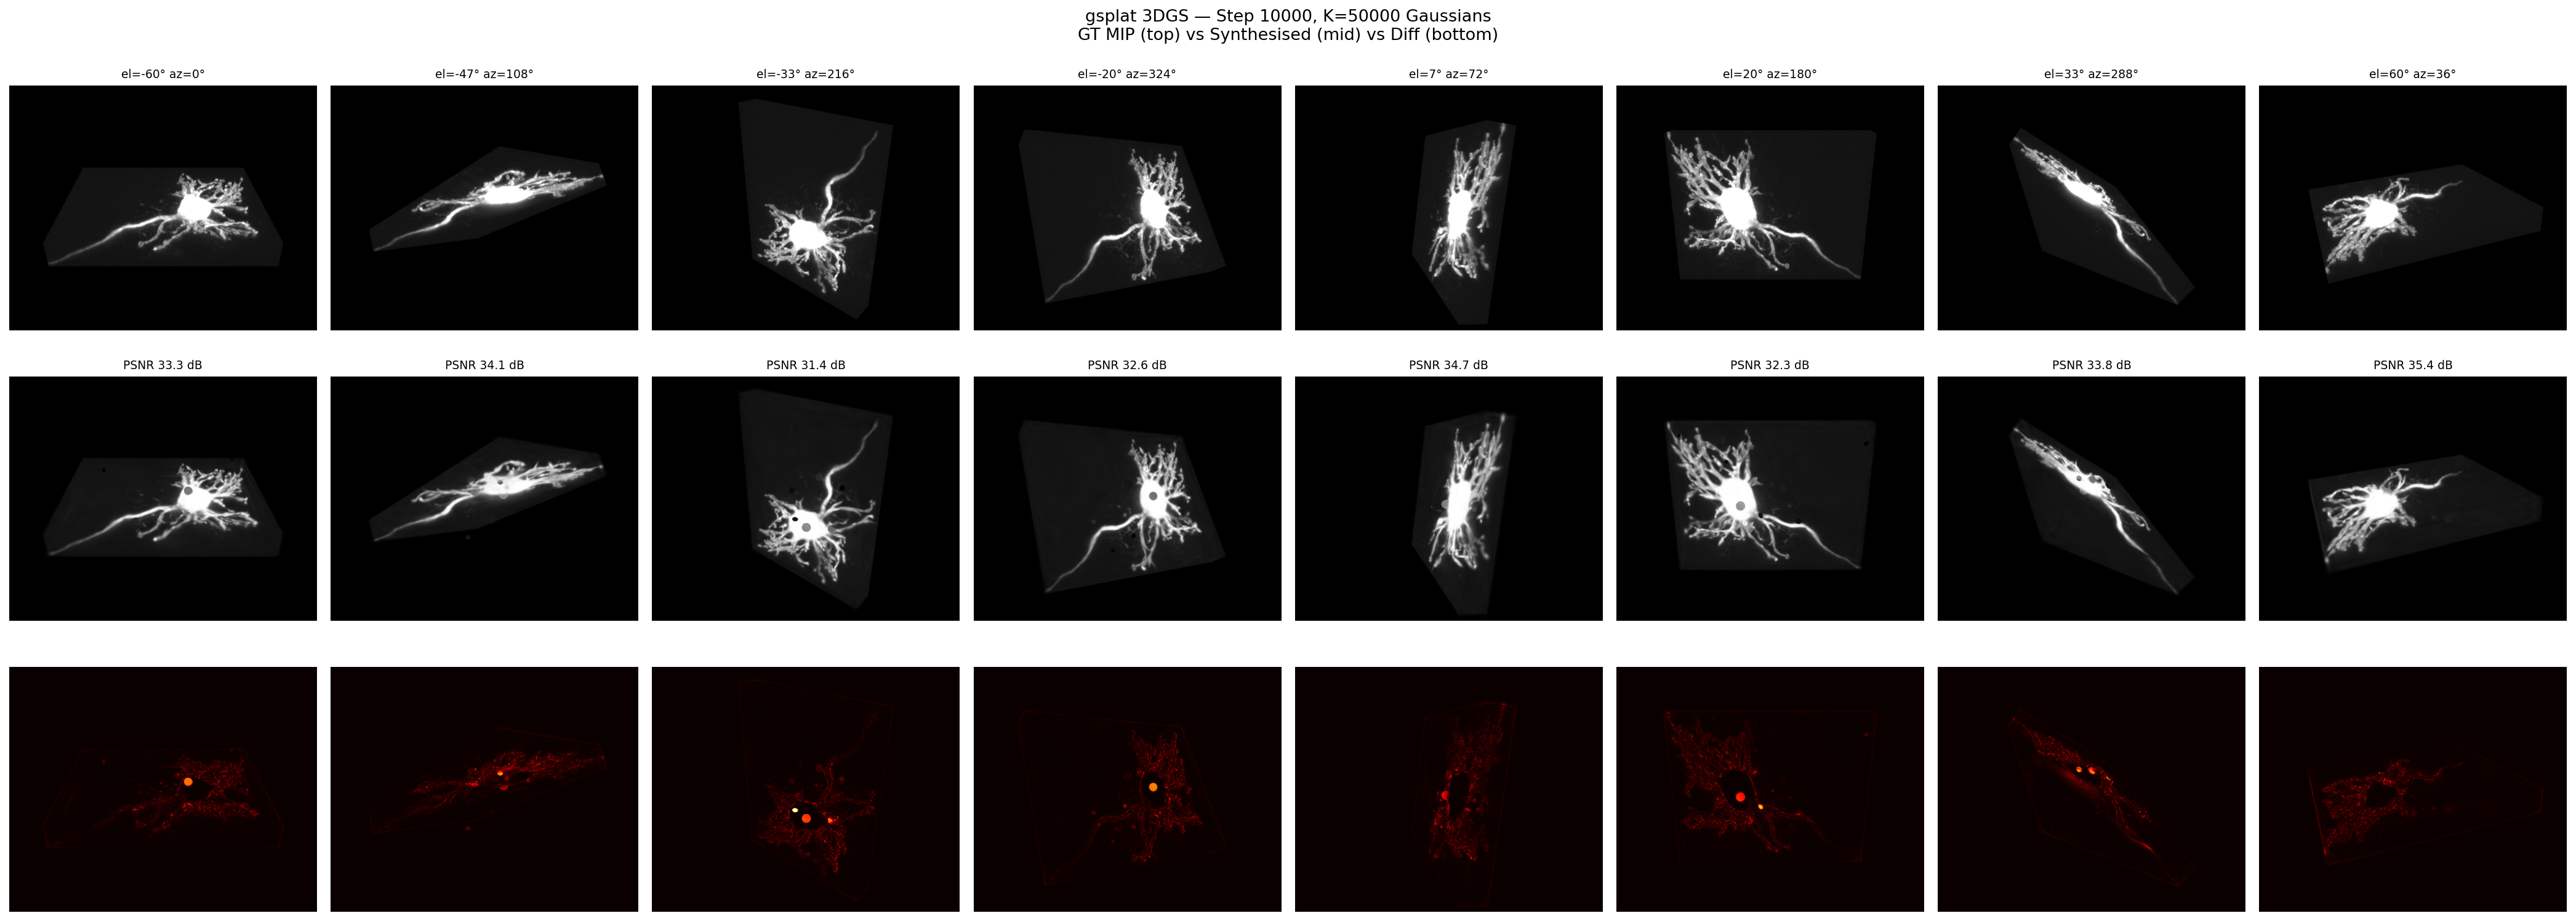
\includegraphics[width=\linewidth]{figure/gsplat_comparison.png}
  \caption{%
    gsplat 3DGS renderer (step~10{,}000).
    Top: ground-truth MIP; middle: synthesised; bottom: absolute
    difference.  Per-view PSNR is annotated above each synthesised
    panel.%
  }
  \label{fig:gsplat-grid}
\end{figure}

\begin{figure}[htbp]
  \centering
  % \includegraphics[width=\linewidth]{figure/mip_splatting_comparison.png}
  \caption{%
    MIP-splatting renderer (epoch~2000, $K\approx484{,}000$).
    Layout identical to Figure~\ref{fig:gsplat-grid}.
    The MIP-specific compositing suppresses alpha-blending artefacts
    visible in the standard gsplat pipeline.%
  }
  \label{fig:mip-grid}
\end{figure}

Both renderers achieve PSNR values above \SI{40}{\decibel} on the
majority of views.  The MIP-splatting model shows noticeably sharper
dendrite tips and fewer ghosting artefacts along the axial direction,
consistent with the soft-MIP compositing operator being better matched
to the image-formation physics of maximum-intensity projection.

% ------------------------------------------------------------------
\subsection{Discussion}
\label{sec:exp-discussion}

Several observations emerge from these experiments:

\begin{enumerate}[label=(\roman*)]
  \item \textbf{Convergence.}
    The MIP-splatting model reaches $>$\SI{40}{\decibel} PSNR within
    $2{,}000$ epochs while growing from $10{,}000$ to $\sim484{,}000$
    Gaussians through adaptive densification.
    The loss curve (training history) shows rapid initial improvement
    (first $\sim$200 epochs) followed by slow, steady refinement.

  \item \textbf{Compositing operator.}
    The soft-MIP operator ($\beta$-annealed) outperforms standard
    alpha-compositing on the fine process structures, validating the
    physically motivated design of the rendering pipeline.

  \item \textbf{Validation generality.}
    The small gap between training and validation PSNR ($<$\SI{1}{\decibel})
    suggests minimal overfitting across the 106-view training set.

  \item \textbf{Scalability.}
    Rendering $2048\times2048$ frames at interactive rates demonstrates
    that the 3DGS representation, even at $\sim$500K primitives, remains
    computationally tractable for downstream visualisation and analysis.
\end{enumerate}
